
%%%%%%%%%%%%%%%%%%%%%%%%%%%%%%%%%%%%%%%%%%%%%%%%%%%%%%%%%
\documentclass[inzynierska]{pwr_wmat_praca_dyplomowa}
\usepackage{graphicx}
\usepackage{ amssymb }
\usepackage{ dsfont }
\usepackage{amsmath}
\usepackage{algpseudocode}
\graphicspath{{C:/Users/micha/Desktop/inzynier/NBA_Simulator/grafika/}} 

\autor{Michał Cerazy}
\tytul{Zastosowanie metod bootstrapowych do prognozowania wyników w zawodach sportowych} 
\tytulang{Application of bootstrap methods to the forecasting of sporting event results}
\opiekun{dr hab.\ inż.\ Krzysztof Burnecki}
\kierunekstudiow{Matematyka Stosowana}
\kierunekstudiowang{Applied Mathematics}
\specjalnosc{--} 
\specjalnoscang{--} 
\streszczenie{Praca dotyczy aktualnego problemu z matematyki stosowanej, a mianowicie stworzenia symulatora ligi NBA przy użyciu znanych technik matematycznych/statystycznych. Celem pracy jest stworzenie symulatora rozgrywek w lidze NBA przy użyciu metod bootstrapowych. Wynikiem pracy będzie oprogramowanie do symulacji rozgrywek w lidze NBA umożliwiające prognozowanie wyników w następnym roku.}
\streszczenieang{Tutaj piszemy krótkie streszczenie pracy w języku angielskim (nie powinno być dłuższe niż 530 znaków).}
\slowakluczowe{tutaj podajemy najważniejsze słowa kluczowe (łącznie nie powinny być dłuższe niż 150 znaków).}  
\slowakluczoweang{tutaj podajemy najważniejsze słowa kluczowe w języku angielskim (łącznie nie powinny być dłuższe niż 150 znaków)}
%%%%%%%%%%%%%%%%%%%%%%%%%%%%%%%%%%%%%%%%%%%%%%%%%%%%%%%%%
% Definicje, lematy, twierdzenia, przykłady i wnioski
% Komendy wywołujące twierdzenia, definicje, itd., 
% czyli 'theorem', 'definition', 'corollary', itd., 
% można zmienić wedle uznania.
\theoremstyle{plain}
\newtheorem{theorem}{Twierdzenie}
\numberwithin{theorem}{chapter}
\newtheorem{lemma}[theorem]{Lemat} 
\newtheorem{corollary}[theorem]{Wniosek}
\newtheorem{fact}[theorem]{Fakt}
\theoremstyle{definition}
\numberwithin{theorem}{chapter}
\newtheorem{definition}[theorem]{Definicja} 
\newtheorem{algorytm}[theorem]{Algorytm}
\newtheorem{pseudokod}[theorem]{Pseudokod algorytmu}
\newtheorem{example}[theorem]{Przykład}
\newtheorem{note}[theorem]{Uwaga}
%%%%%%%%%%%%%%%%%%%%%%%%%%%%%%%%%%%%%%%%%%%%%%%%%%%%%%%%%
\begin{document}
\frontmatter
\maketitle
\mainmatter
\tableofcontents
%\listoffigures
%\listoftables

{\backmatter \chapter{Wstęp}}
%We wstępie zapowiadamy, o czym będzie praca. Próbujemy zachęcić czytelnika do dalszej lektury, np. krótko informując, dlaczego wybraliśmy właśnie ten temat i co nas w nim zainteresowało.
Dzięki powszechnemu dostępowi do internetu i rozpowszechnieniu kultury masowej amerykańska liga koszykarska NBA zyskała popularność na całym świecie, przyciągając do siebie najlepszych graczy i masy fanów. Z powodu nieprzewidywalności i złożoności tego sportu podejmowano wiele prób przewidywania wyników rozgrywek, które często toczyły się inaczej, niż by zakładano (najlepszym tego przykładem może być sezon 2003/2004, kiedy to nisko notowani Detroit Pistons pokonali faworytów w postaci Los Angeles Lakers). Trudność w przewidzeniu wyników wynika bezpośrednio z zasad ligi --- dozwolone są w niej wymiany zawodników między klubami, liczne i często katastrofalne kontuzje, czy nabory do ligi, w których najgorsze drużyny mają pierwszeństwo wyboru nowych zawodników chcących dołączyć do NBA (z tego powodu wiele organizacji celowo przegrywa mecze w celu wylosowania najwyższych miejsc w naborze). Najlepsi analitycy sportowi podejmują starania badać każdy aspekt gry i jego wpływ na przebieg meczu. Niemal wszystkie zaproponowane dotąd modele symulacji rozgrywek opierają się na statystykach zawodników, ich wpływie na atak i obronę, oraz udziale w zwycięstwach. Celem tej pracy inżynierskiej jest próba przewidzenia rezultatów wybranego sezonu ligi NBA przy pomocy bardzo prostego modelu, używając wyłącznie informacji o wynikach poszczególnych drużyn w poprzednich sezonach --- indywidualny wpływ graczy na przebieg spotkań nie jest rozpatrywany. Na potrzeby tego zadania zaprojektowano kilka algorytmów opierających się na metodzie \textbf{bootstrapu parametrycznego}, sprawdzono ich skuteczność dla kilku wybranych sezonów w zależności od okresu używanych danych i nadawania wag, a następnie przy pomocy najskuteczniejszych modeli dokonano predykcji wyników trwającego sezonu 2018/2019. 

\chapter{Opis ligi NBA, jak wyglada sezon}\label{rodzial1}
National Basketball Association (NBA) została założona 6 czerwca 1946 roku. Pierwotnie była znana jako Basketball Association of Americai składała się z 11 zespołów, a swoją obecną nazwę zyskała w roku 1949, kiedy to wchłonęła rywalizującą National Basketball League. Od 2004 roku w NBA gra 30 zespołów, 29 ze Stanów Zjednoczonych i 1 z Kanady. Liga podzielona jest na dwie konferencje po 15 drużyn, te natomiast składają się z dywizji po 5 organizacji. Szczegółowy podział konferencje i dywizje, oraz nazwy wszystkich drużyn zawarte zostały w Tabelach \ref{tabela_wschod} i \ref{tabela_zachod}, natomiast dokładne rozmieszczenie na mapie kontynentu znajduje się na Rysunku \ref{mapa_stany}.

\begin{figure}[t]
	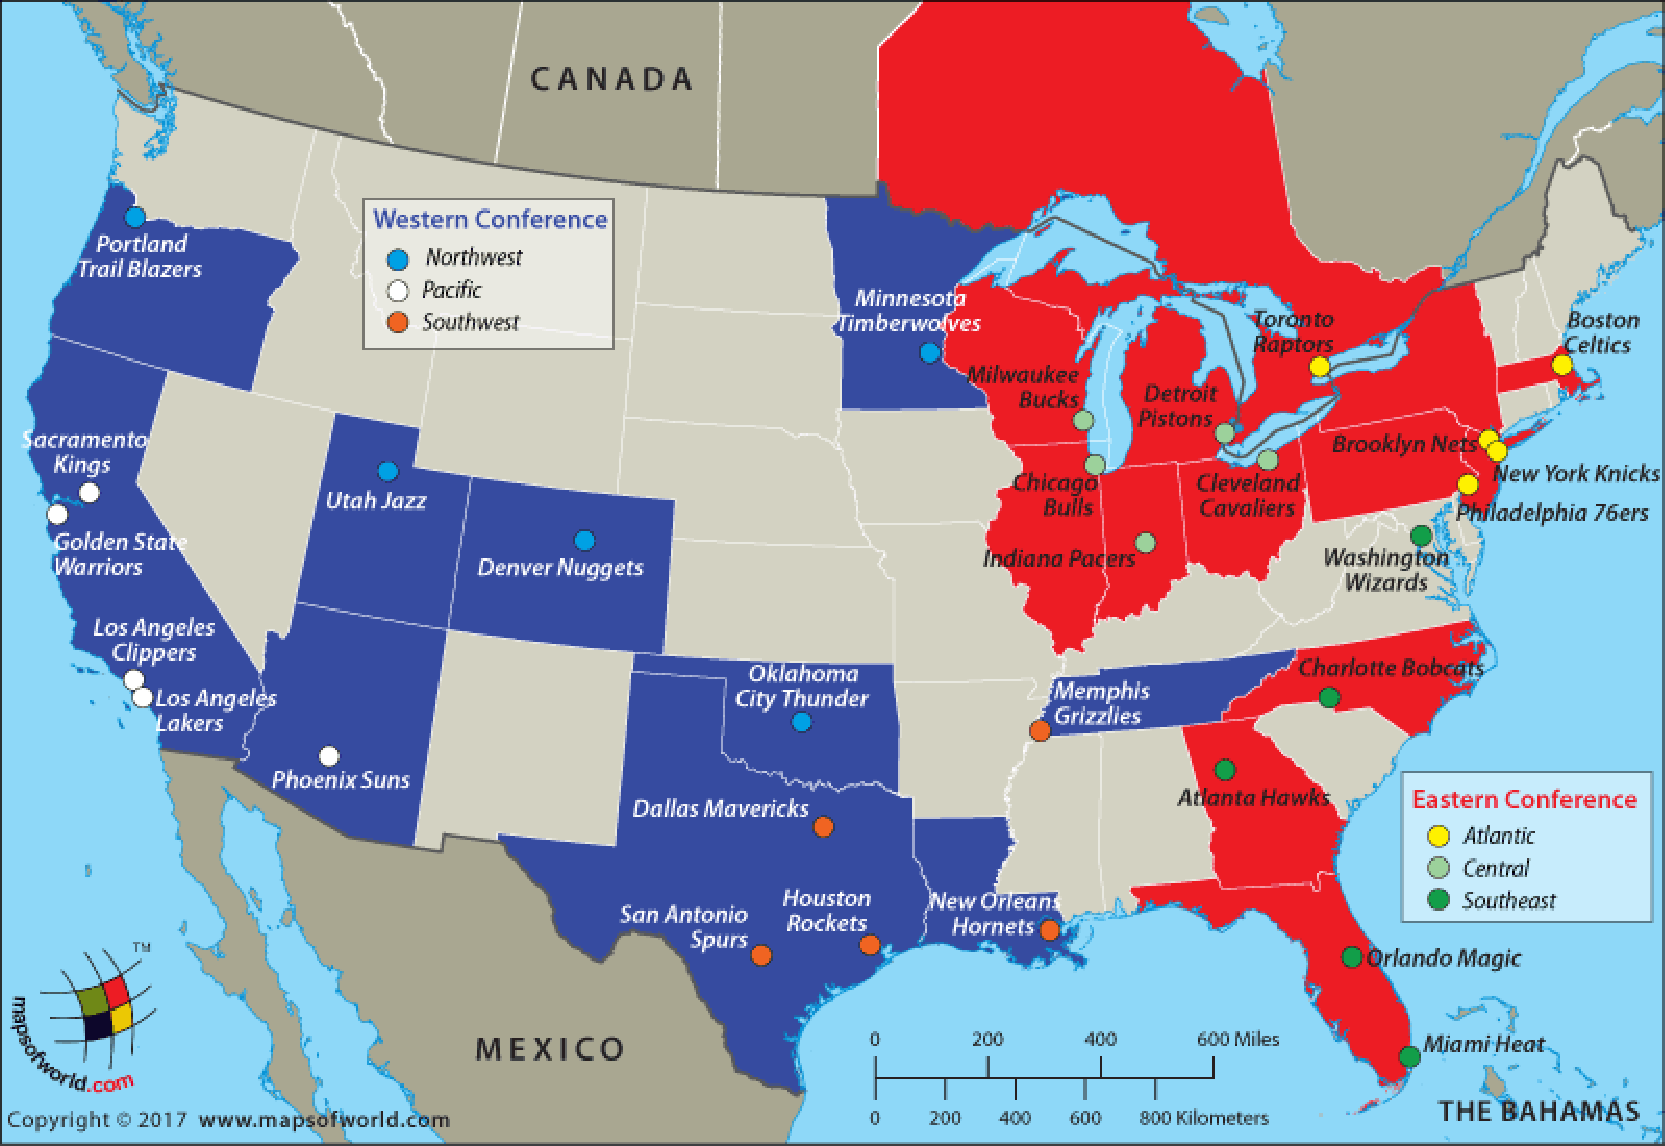
\includegraphics[width=16cm]{conf_map.pdf}
	\caption{Rozmieszczenie drużyn NBA}\label{mapa_stany}
	\centering
\end{figure}

\begin{table}[]
\begin{tabular}{ |p{5cm}|p{5cm}|p{5cm}|  }
	\hline
	\multicolumn{3}{|c|}{\textbf{Konferencja Wschodnia}} \\
	\hline
	\textbf{Atlantic Division}& \textbf{Southeast Division}&\textbf{Central Division}\\
	\hline
	Boston Celtics (BOS)& Atlanta Hawks (ATL)&Chicago Bulls (CHI)\\\hline
	Brooklyn Nets (BRK)&Charlotte Hornets (CHO)&Cleveland Cavaliers (CLE)\\\hline
	New York Knicks (NYK)&Miami Heat (MIA)&Detroit Pistons (DET)\\\hline
	Philadelphia 76ers (PHI)&Orlando Magic (ORL)&Indiana Pacers (IND)\\\hline
	Toronto Raptors (TOR)&Washington Wizards (WAS)&Milwaukee Bucks (MIL)\\\hline
	\hline
\end{tabular}
\caption{Drużyny Konferencji Wschodniej}\label{tabela_wschod}
\end{table}
\begin{table}[]
\begin{tabular}{ |p{5.8cm}|p{5.4cm}|p{5.6cm}|  }
	\hline
	\multicolumn{3}{|c|}{\textbf{Konferencja Zachodnia}} \\
	\hline
	\textbf{Northwest Division}& \textbf{Southwest Division}&\textbf{Pacific Division}\\
	\hline
	Denver Nuggets (DEN)& Dallas Mavericks (DAL)&Golden State Warriors (GSW)\\\hline
	Minnesota Timberwolves (MIN)&Houston Rockets (HOU)&Los Angeles Clippers (LAC)\\\hline
	Oklahoma City Thunder (OKC)&Memphis Grizzlies (MEM)&Los Angeles Lakers (LAL)\\\hline
	Portland Trail Blazers (POR)&New Orleans Pelicans (NOP)&Phoenix Suns (PHX)\\\hline
	Utah Jazz (UTA)&San Antonio Spurs (SAS)&Sacramento Kings (SAC)\\
	\hline
\end{tabular}
\caption{Drużyny Konferencji Zachodniej}\label{tabela_zachod}
\end{table}

Dodatkowo, od 2004 roku niektóre kluby zmieniły swoje nazwy lub lokalizacje. W niektórych historycznych zestawieniach lub zbiorach danych mogą widnieć jako (podane w formacie nazwa obecna --- poprzednia):
\begin{itemize}
	\item Charlotte Hornets --- Charlotte Bobcats
	\item Brooklyn Nets --- New Jersey Nets
	\item Oklahoma City Thunder --- Seattle SuperSonics
	\item New Orleans Pelicans --- New Orleans Hornets
\end{itemize}

Sezon w NBA składa się z dwóch części: zasadniczej i następującej po niej pucharowej (playoffs). W sezonie zasadniczym każda drużyna rozgrywa 82 mecze, grając z każdym innym zespołem od 2 do 4 gier. Terminarz wyznaczany jest wedle następujących reguł:
\begin{enumerate}
	\item drużyny z różnych konferencji grają ze sobą 2 spotkania (1 na wyjedzie i 1 na własnym boisku),
	\item drużyny z tej samej dywizji grają ze sobą 4 spotkania (2 na wyjedzie i 2 na własnym boisku),
	\item drużyny z tej samej konferencji oraz różnych dywizji grają ze sobą 3 albo 4 spotkania (przynajmniej po jednym na wyjedzie i własnym boisku).
\end{enumerate}
Mecze koszykówki nie mogą zakończyć się remisem (w razie remisu po regulaminowym czasie gry rozgrywa się dogrywki aż do wyłonienia zwycięzcy).
Po zakończeniu sezonu następuje wspomniana wyżej faza pucharowa; wchodzi do niej po 8 najlepszych zespołów z każdej konferencji (w razie takiej samej ilości zwycięstw dla obu zespołów decydują mecze bezpośrednie pomiędzy nimi). W tej fazie drużyny grają ze sobą maksymalnie 7 meczów, czyli zespół, który pierwszy wygra 4 mecze, przechodzi do następnego etapu. W fazie Playoff jasno zdefiniowane są lokalizacje odgrywania spotkań --- lepszy bilans zwycięstw w sezonie zasadniczym skutkuje przewagą parkietu. Seria spotkań grana jest w formacie 2–2–1–1–1, czyli mecze numer 1, 2, 5 i 7 grane są u lepszej z drużyn. Przy doborze przeciwników w tej fazie bierze się pod uwagę pozycję w tabeli konferencji: drużyna z miejsca pierwszego gra z zespołem o ósmym bilansie w danej konferencji, druga z siódmą, i tak dalej. Zwycięzca serii przechodzi do następnego etapu z czterema drużynami, po którym następują finały konferencji --- najlepsze drużyny ze swoich konferencji spotykają się w finałach NBA. Dla lepszego zrozumienia systemu rozgrywek pucharowych na Rysunku \ref{po_tree} zamieszczono tzw. ,,drzewko Playoff''.  

\begin{figure}[t]
	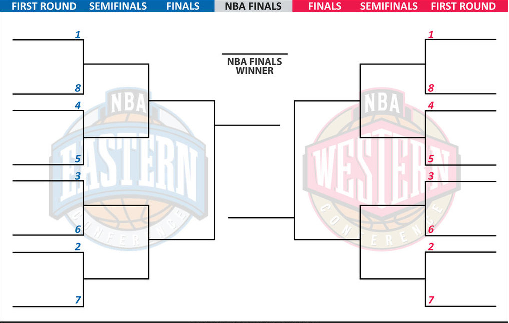
\includegraphics[width=16cm]{po_tree.pdf}
	\caption{Drzewko Playoff}\label{po_tree}
	\centering
\end{figure}

Wyniki z sezonu regularnego 2014/2015 prezentują się następująco:

\begin{table}[]
	\centering
\begin{tabular}{|c|c|c|}
	\hline
	\textbf{Drużyna}      & \textbf{Zwycięstwa w sezonie 14/15} & \textbf{Zwycięstwa w sezonie 17/18} \\ \hline
	Atlanta Hawks & 60 & 24\\ \hline
	Boston Celtics & 40 & 55\\ \hline
	Brooklyn Nets & 38 & 28\\ \hline
	Charlotte Hornets & 33 & 36\\ \hline
	Chicago Bulls & 50 & 27\\ \hline	
	Cleveland Cavaliers & 53 & 50\\ \hline
	Dallas Mavericks & 50 & 24\\ \hline	
	Denver Nuggets & 30& 46\\ \hline
	Detroit Pistons & 32 & 39\\ \hline
	Golden State Warriors & 67 & 58\\ \hline
	Houston Rockets & 56 & 65 \\\hline
	Indiana Pacers & 38 & 48 \\\hline
	Los Angeles Clippers & 56 & 42\\ \hline
	Los Angeles Lakers & 21 & 35\\ \hline
	Memphis Grizzlies & 55 & 22\\ \hline
	Miami Heat & 37 & 44 \\\hline
	Milwaukee Bucks & 41 & 44\\ \hline
	Minnesota Timberwolves & 16 & 47\\ \hline
	New Orleans Pelicans & 45 & 48\\ \hline
	New York Knicks & 17 & 29\\ \hline
	Oklahoma City Thunder & 45 & 48\\ \hline
	Orlando Magic & 25 & 17\\ \hline
	Philadelphia 76ers & 18 & 52\\ \hline
	Phoenix Suns & 39 & 21 \\\hline
	Portland Trail Blazers & 51 & 49\\ \hline	
	Sacramento Kings & 29 & 27\\ \hline
	San Antonio Spurs & 55 & 47\\ \hline
	Toronto Raptors & 49 & 59\\ \hline
	Utah Jazz & 38 & 48 \\\hline
	Washington Wizards & 46 & 43\\ \hline
\end{tabular}
\caption{Liczby zwycięstw drużyn w wybranych sezonach}\label{tabela_wygrane_rzeczywiste}	
\end{table}

\begin{table}[]
	\centering
	\begin{tabular}{ |p{5cm}|p{5cm}|c|  }
		\hline
		\textbf{Zwycięzca}& \textbf{Przegrany} &\textbf{Wynik}\\\hline		
		\multicolumn{3}{|c|}{Eastern Conference First Round} \\\hline
		Atlanta Hawks& Brooklyn Nets &4-2\\\hline
		Chicago Bulls& Milwaukee Bucks&4-2\\\hline
		Cleveland Cavaliers& Boston Celtics &4-0\\\hline
		Washington Wizards& Toronto Raptors&4-0\\\hline
		\multicolumn{3}{|c|}{} \\\hline
		
		\multicolumn{3}{|c|}{Western Conference First Round} \\\hline
		Golden State Warriors &New Orleans Pelicans &4-0\\\hline
		Houston Rockets& Dallas Mavericks&4-1\\\hline
		Los Angeles Clippers& San Antonio Spurs &4-3\\\hline
		Memphis Grizzlies& Portland Trail Blazers&4-1\\\hline
		\multicolumn{3}{|c|}{} \\\hline

		\multicolumn{3}{|c|}{Eastern Conference Semifinals} \\\hline
		Atlanta Hawks& Washington Wizards &4-2\\\hline
		Cleveland Cavaliers& Chicago Bulls&4-2\\\hline
		\multicolumn{3}{|c|}{} \\\hline
		
		\multicolumn{3}{|c|}{Western Conference Semifinals} \\\hline
		Golden State Warriors& Memphis Grizzlies &4-2\\\hline
		Houston Rockets& Los Angeles Clippers&4-3\\\hline
		\multicolumn{3}{|c|}{} \\\hline
		
		\multicolumn{3}{|c|}{Eastern Conference Finals} \\\hline
		Cleveland Cavaliers& Atlanta Hawks&4-0\\\hline
		\multicolumn{3}{|c|}{} \\\hline
		
		\multicolumn{3}{|c|}{Western Conference Finals} \\\hline
		Golden State Warriors& Houston Rockets&4-1\\\hline
		\multicolumn{3}{|c|}{} \\\hline
		
		\multicolumn{3}{|c|}{Finals} \\\hline
		Golden State Warriors& Cleveland Cavaliers &4-2\\\hline
	\end{tabular}
\caption{Rozgrywki pucharowe w 2015 roku}\label{tabela_playoffs2015}
\end{table}

\chapter{Teoria, matematyka}
%, estymacja, boxplot, zmienna losowa, symulowanie z dystrybuanty
%wartość oczekiwana, CZY BADAMY NORMALNOŚĆ? test shapiro-wilka, gęstość rozkładu, rozklad normalny, qqplot?

\section{Rozkład jednostajny}
Ciągła zmienna losowa $X$ ma rozkład jednostajny o parametrach $a$ i $b$, takich że $a,b\in \mathds{R}$ oraz $a<b$, oznaczany jako $\mathcal{U}(a,b)$ wtedy, gdy jej gęstość jest postaci
\begin{equation}
f(x)=\frac{1}{b-a}\mathds{1}_{(a,b)}(x).
\end{equation}
Wartość oczekiwana wynosi
\begin{equation}
E(X)=\frac{a+b}{2},
\end{equation}
natomiast wariancja jest równa
\begin{equation}
Var(X)=\frac{(b-a)^2}{12}.
\end{equation} 
Funkcja charakterystyczna tego rozkładu wyrażana jest wzorem
\begin{equation}
\phi(t)=\frac{e^{itb}-e^{ita}}{(b-a)it}.
\end{equation}
W przypadku, gdy zmienna losowa $X$ posiada ciągłą dystrybuantę $F(x)$, to $U=F(x)$ ma rozkład $\mathcal{U}(0,1).$

\section{Generatory liczb pseudolosowych rozkładu jednostajnego} %(str 427)
Załóżmy, że $F$ to dystrybuanta rozkładu normalnego $\mathcal{U}(0,1)$. Podczas generowania ciągu zbliżonego do realizacji rozkładu jednostajnego zazwyczaj stosuje się następującą metodę: wybierzmy funkcję $G$ określoną i mająca wartości na odcinku $[0,1]$, o wartości początkowej $u_0 \in [0,1]$, i zdefiniujmy
\begin{equation}
	u_1=G(u_0), \,\, u_2=G(u_1), \,\, \dots, \,\,u_i=G(u_{i-1}), \,\, i=1,\,2,\,\dots 
\end{equation}
Znając postać funkcji $G$ i początkową wartość $u_0$ możliwe jest ponowne wygenerowanie każdego elementu zdefiniowanego powyżej ciągu. Prowadzi to do następującej definicji:
\begin{definition}
	Generator liczb pseudolosowych z rozkładu jednostajnego $\mathcal{U}(0,1)$ to taki algorytm dla funkcji $G$ o wartości startowej $u_0 \in [0,1]$, który wyznacza wartości $u_n$, mając przy okazji podaną własność: dla każdego $n$, wygenerowane $u_1,u_2,\dots,u_n$ oddają zachowanie próby losowej $U_1,U_2,\dots,U_n \sim \mathcal{U}(0,1)$ (popularne testy nie odrzucają hipotezy, wedle której $u_1,u_2,\dots,u_n$ to realizacja próby $U_1,U_2,\dots,U_n \sim \mathcal{U}(0,1)$).
\end{definition}

\section{Metoda Monte Carlo}
Załóżmy, że $\theta$ to parametr zmiennej losowej $X$ oraz można go przedstawić jako $\theta=Eh(X)$, przy czym $h$ to pewna znana funkcja, dodatkowym założeniem jest, że można wygenerować próbę o rozkładzie $X$. 
\begin{definition}
	Niech $X_1,X_2,\dots,X_m$ będzie próbą pseudolosową pewnego rozkładu $X$ dla pewnego $m$. Średnia $\bar{h}=m^{-1}(h(X_1)+h(X_2)+\dots +h(X_m))$ nazywana jest \textbf{estymatorem $Eh(X)=\theta$ wyznaczonym metodą Monte Carlo}.
\end{definition}
Można zauważyć, że $\bar{h}$ to średnia próbkowa próby $h(X_1),h(X_2),\dots ,h(X_m)$, użycie jej do oszacowania parametru $\theta$ jest możliwe dzięki prawu wielkich liczb. Głównym problemem tego zagadnienia jest estymacja parametru $\theta$, który nie musi posiadać interpretacji probabilistycznej. Całość tej metody opiera się na generowaniu próby losowej lub pseudolosowej rozkładu jednostajnego , zastosowaniu funkcji $h$ do przekształcenia elementów tej próby, a następnie wyznaczeniu estymatora $\bar{h}$ parametru $\theta$. 
W celu dokładnego opisania metody posłużmy się przykładem: obliczmy
\begin{equation}
	\theta:=\int_{0}^{1}g(x)\,dx.
\end{equation}
W przypadku, gdy nie jesteśmy w stanie policzyć tej całki analitycznie, pozostaje nam zastosowanie metod numerycznych lub symulacyjnych. Algorytm szacowania parametru $\theta$ przy użyciu metody Monte Carlo:
\begin{enumerate}
	\item wygeneruj $U_1,U_2,\dots, U_n \sim \text{IID}\,\,\,\, \mathcal{U}(0,1)$,
	\item oszacuj $\theta$ korzystając z
	\begin{equation}
		\hat{\theta_n}:= \frac{g(U_1)+g(U_2)+\dots+g(U_n)}{n}.
	\end{equation}
\end{enumerate} 

Modelowanie przy pomocy metody Monte Carlo jest przydatne przy badaniu skomplikowanych procesów losowych, które można rozbić na dwie kategorie. Pierwsza skupia w sobie systemy, w których proces jest sprecyzowany, ale poprzez jego złożoność trudno obliczyć jego parametry teoretyczne. Druga kategoria to eksperymenty losowe o modelu matematycznym trudnym do skonstruowania --- dzięki metodzie Monte Carlo można dokonać ich klasyfikacji generując wyniki modelowe, po czym przyrównać je z danymi eksperymentalnymi. Omawiana w następnym Rozdziale metoda bootstrap w swoich założeniach wywodzi się z symulacji Monte Carlo.

\section{Zasada bootstrap}
%In statistics, bootstrapping is any test or metric that relies on random sampling with replacement.
Próba bootstrap to metoda służąca do oceny rozkładu pewnego estymatora (na przykład wariancji)  używając wielokrotnych symulacji opartych na znanej realizacji jego rozkładu.  
 Narzędzie to zostało stworzone przez Bradleya Efrona i opublikowane w artykule ,,Bootstrap methods: another look at the jackknife'' z 1979 roku. Załóżmy, że $x_1, x_2 \dots x_n$ to realizacja pewnej próby losowej, a $\hat{F}$ jest dystrybuantą empiryczną tej próby. Dystrybuanta $\hat{F}$ to znane przybliżenie pewnego nieznanego rozkładu $F$, dlatego też rozkład $\hat{\Theta}$ estymować będziemy przy pomocy $\hat{F}$, czyli dokonamy oceny rozkładu estymatora $\hat{\Theta}$ w oparciu o generowanie prób z rozkładu $\hat{F}$. 
\begin{definition}
	Próba losowa $X^* = (X_1^*, X_2^*, \dots, X_n^*)$ o rozkładzie $\hat{F}$ dla ustalonej realizacji $x = (x_1, x_2, \dots, x_n)$ nazywana jest \textbf{próbą bootstrap}.
\end{definition}
Otrzymywanie realizacji próby bootstrap bazuje na wykonaniu $n$-krotnego losowania ze zwracaniem elementów próby pierwotnej, tak więc losowość w próbie $X^*$ polega na losowym wyborze elementu $x_1, x_2, \dots, x_n$. W ten sposób powstaje populacja, w której każda zmienna $X_i^*$ jest niezależna od pozostałych, oraz z jednakowym prawdopodobieństwem  przyjmuje dowolną wartość próby. Efron wykazał, że rozkład $T(X^*)$ dla ustalonych $x_1, x_2, \dots, x_n$ ma kształt zbliżony do rozkładu $T(X)$, ponadto rozkład statystyki $(T(X^*)-\hat{\Theta})$ jest bliski rozkładowi statystyki $(T(X)-\Theta)$. Dzięki temu można dokonać oceny rozkładu $\Theta=T(X)$ wykonując poniższe kroki:
\begin{enumerate}
	\item dokonaj losowania niezależnych prób bootsrap $X_1^*, X_2^*, \dots, X_k^*$ korzystając z realizacji $x_1, x_2, \dots, x_n$,
	\item wyznacz $\Theta_1^*=T(X_1^*)-\hat{\Theta}$, $\Theta_2^*=T(X_2^*)-\hat{\Theta}$, \dots, $\Theta_k^*=T(X_k^*)-\hat{\Theta}$.
\end{enumerate}
Otrzymany w ten sposób rozkład $(\Theta_1^*, \Theta_2^*, \dots, \Theta_k^*)$ to przybliżenie rozkładu błędów estymacji $\hat{\Theta}-\Theta$ przy pomocy statystyki $T$. Histogram tego rozkładu nazywany jest estymatorem rozkładu $\hat{\Theta}$ otrzymanym metodą bootstrap. Dla zadowalającego przybliżenia rozkładu $(T(X^*)-\hat{\Theta})$ wymagane jest przynajmniej $k=1000$ prób bootstrap, a im większa ich ilość, tym dokładniejsze oszacowanie.  

\subsection{Bootstrap parametryczny}
Założenia bootstrapu parametrycznego są podobne do bootstrapu klasycznego --- jedyną różnicą jest fakt, że zamiast symulowania niezależnych prób bootstrapowych z dystrybuanty empirycznej, generowane są niezależne próby z rozkładu pewnego parametrycznego modelu. 
W tym przypadku do danych dopasowany jest pewien model teoretyczny (często przy pomocy metody największej wiarygodności), a próby liczb losowych generowane są z owego dopasowanego modelu. Proces symulowania tak zdefiniowanej proby przebiega podobnie do innych procesów bootstrapowych, przy czym wielkość takiej próby zazwyczaj odpowiada rozmiarowi oryginalnego zbioru danych. Prowadzi to do następującej definicji:
\begin{definition}
	Próbę bootstrap, której nieznany rozkład $F$ można przybliżyć pewnym znanym rozkładem parametrycznym $\hat{F}$ nazywamy \textbf{parametryczną próbą bootstrap}. 
\end{definition}
%In this case a parametric model is fitted to the data, often by maximum likelihood, and samples of random numbers are drawn from this fitted model. Usually the sample drawn has the same sample size as the original data. Then the quantity, or estimate, of interest is calculated from these data. This sampling process is repeated many times as for other bootstrap methods. The use of a parametric model at the sampling stage of the bootstrap methodology leads to procedures which are different from those obtained by applying basic statistical theory to inference for the same model.\\
%The theory of the parametric bootstrap is quite similar to that of the nonparametric bootstrap, the only difference is that instead of simulating bootstrap samples that are IID from the empirical distribution (the nonparametric estimate of the distribution of the data) we simulate bootstrap samples that are IID from the estimated parametric model.
 
\chapter{Metodologia, algorytmy}\label{rodzial_algorytmy}
Czy znając wyniki zakończonych rozgrywek jesteśmy w stanie przewidzieć rezultaty przyszłych zawodów?
\\
Dane, które będą wykorzystywane do symulacji sezonu zostały zebrane ze strony sportowej basketballreference.com.
\\
Na potrzeby tej pracy zebrano wyniki starć pomiędzy drużynami począwszy od sezonu 2004/2005 aż do 2017/2018. Początkowo symulowano rozgrywki sezonów 2014/2015 oraz 2017/2018 w celu wybrania najlepszego modelu, a następnie skorzystano z niego, aby przewidzieć wyniki rozgrywek we wciąż trwającym sezonie 2018/2019.
Posiadając ilość wygranych jednej drużyny z drugą na przestrzeni lat dokonano następujących transformacji danych:
\\
W zależności od interwału czasowego, jaki będziemy rozpatrywać, zebrano wyniki w określonych rozgrywkach (na przykład, przy wyznaczaniu wyników sezony 2014/2015 i interwale 5 lat, używać będziemy danych z lat 2009 do 2014). Dzięki uzyskanej w ten sposób liczbie wygranych w możemy stosunek zwycięstw do porażek dla wybranych zespołów (przykład: Boston Celtics i Atlanta Hawks grały ze sobą 10 razy, Jastrzębie wygrały zaledwie 4 razy, dlatego też w starciu z Celtami ich stosunek wygranych do przegranych wynosi $0.4$). Po zastosowaniu tej metody dla wszystkich zespołów uzyskano macierz o rozmiarze 30 wierszy i kolumn zawierającą prawdopodobieństwa na wygraną z każdym zespołem w lidze.
\\
Podczas prób symulacji dokonano intuicyjnego założenia, wedle którego największy wpływ na postawę sezonu mają rozgrywki bezpośrednio go poprzedzające. W tym celu dobrano system wag --- z powodu dynamicznych zmian w lidze, najstarsze sezony otrzymują najmniejszą rangę, która stopniowo zwiększa się, im bliżej do zawodów rozpatrywanych w symulacji. Ważona ilość zwycięstw $Z_i$ $i-$tej drużyny $D_i$ z $j-$tą drużyną $D_j$ wynosi
\begin{equation}
	Z_{ij} = \sum_{k=1}^{n} (1+x\cdot k)\cdot R_{ijk}, 
\end{equation}
gdzie $n$ to ilość sezonów, z których zaciągamy dane, $x$ ustalona waga kolejnych rozgrywek, a $R_{ijk}$ to wynik starć drużyny $D_i$ z drużyną $D_j$ w $k-$tym sezonie. Podczas testowania skuteczności modeli dobierano różne wagi w celu znalezienia tego zwracającego najlepsze predykcje.    
\\
Podczas symulacji program przechodzi przez dokładnie określony terminarz rozgrywek --- drużyna gra z przeciwnikiem tyle razy, ile spotkań wyznaczono w rozkładzie. Algorytmy losowania opisano szczegółowo w Rozdziale \ref{rodzial1}.
\\
Każdy spośród zaproponowanych w tej pracy modeli został przeanalizowany pod względem okresu pobieranych danych oraz wag wpływających na istotność poszczególnych sezonów. Wszystkie symulacje wykonano 10000 razy.
\\
5, 10 lat
\\
k=0, k=0.5, k=1

\section{Modele bootstrapowe}

\subsection{Model uśredniony}
Pierwszy ze stworzonych modeli polega na obliczeniu ogólnego stosunku zwycięstw do porażek dla każdej drużyny w wybranym okresie --- wszystkie wygrane zespołu zostają podzielone przez łączną liczbę rozegranych spotkań, wynikiem czego jest liczba z przedziału $[0,1]$ określana jako $P_{i}$, gdzie $i$ to $i-$ta drużyna. Schemat symulowania wyników spotkań między drużynami wygląda następująco:

\begin{algorytm} \textbf{Algorytm modelu uśrednionego}
	\begin{enumerate}
	\item wstaw liczniki zwycięstw drużyn $B_1= 0,B_2= 0,\dots, B_{30}= 0$
	\item dla $i=1$, $i=2$, \dots $i=30$: 
	\begin{enumerate}
		\item dla $j=i$, $j=i+1$, \dots $j=30$: 
		\begin{enumerate}
			\item znajdź drużyny $D_i$ i $D_j$
		\item odczytaj średnie ilości zwycięstw $W_i$ i $W_j$ dla drużyn $D_i$ i $D_j$ 
		\item wyznacz prawdopodobieństwo zwycięstwa $W_{ij}$ przez drużynę  $D_i$ równe $W_{ij}=\frac{W_i}{W_i + W_j}$   
		\item w terminarzu znajdź liczbę spotkań $S_{ij}$ pomiędzy drużynami $D_i$ i $D_j$
		\item wykonaj $S_{ij}$ razy:
			\begin{enumerate}
				\item symuluj liczbę $U$ z rozkładu jednostajnego $\mathcal{U}\sim U[0,1]$ 
			\item jeżeli $W_{ij} \leq U,$ to zwiększ licznik zwycięstw $B_i=B_i+1$, w przeciwnym razie zwiększ licznik zwycięstw $B_j=B_j+1$
			\end{enumerate}
		\end{enumerate}
	\end{enumerate}
\end{enumerate}
\end{algorytm} 
 
\begin{pseudokod}
	\begin{algorithmic}[1]
		\State $B_1\gets 0,B_2\gets 0,\dots, B_{30}\gets 0$
		\State $i\gets 1$
		\While{$i\leq 30$}
		\For{$j\gets i$ to 30}
		\State znajdź drużyny $D_i$ i $D_j$
		\State znajdź $W_i$ i $W_j$ 
		\State $W_{ij}\gets\frac{W_i}{W_i + W_j}$
		\State znajdź liczbę spotkań $S_{ij}$ pomiędzy $D_i$ i $D_j$
		\For{$p\gets1$ to $S_{ij}$}
		\State $U\sim \mathcal{U}[0,1]$
		\If {$W_{ij} \leq U$}
		\State $B_i \gets B_i+1$
		\Else
		\State $B_j \gets B_j+1$
		\EndIf
		\EndFor
		\EndFor
		\State $i\gets i+1$
		\EndWhile
	\end{algorithmic}
\end{pseudokod}

\subsection{Model rywalizacji}
Drugi z zaproponowanych modeli zakłada zwracanie uwagi na historyczne wyniki przeciwko konkretnej drużynie. W zawodowym sporcie niejednokrotnie można trafić na zażarte rywalizacje między dwoma klubami lub zwykłą łatwość w pokonaniu szczególnego przeciwnika. Algorytm symulowania wyników spotkań między drużynami wygląda następująco:

\begin{algorytm} \textbf{Algorytm modelu rywalizacji}
	\begin{enumerate}
		\item wstaw liczniki zwycięstw drużyn $B_1= 0,B_2= 0,\dots, B_{30}= 0$
		\item dla $i=1$, $i=2$, \dots $i=30$: 
		\begin{enumerate}
			\item dla $j=i$, $j=i+1$, \dots $j=30$: 
			\begin{enumerate}
				\item znajdź drużyny $D_i$ i $D_j$
				\item odczytaj z macierzy wyników stosunek zwycięstw $W_{ij}=\frac{Z_{ij}}{Z_{ij}+Z_{ji}}$ drużyny $D_i$ przeciw drużynie $D_j$   
				\item w terminarzu znajdź liczbę spotkań $S_{ij}$ pomiędzy drużynami $D_i$ i $D_j$
				\item wykonaj $S_{ij}$ razy:
				\begin{enumerate}
					\item symuluj liczbę $U$ z rozkładu jednostajnego $\mathcal{U}\sim U[0,1]$ 
					\item jeżeli $W_{ij} \leq U,$ to zwiększ licznik zwycięstw $B_i=B_i+1$, w przeciwnym razie zwiększ licznik zwycięstw $B_j=B_j+1$
				\end{enumerate}
			\end{enumerate}
		\end{enumerate}
	\end{enumerate}
\end{algorytm} 


\subsection{Model symulacji spotkań fazy pucharowej}
Po symulacji całego sezonu, czyli 1230 spotkań, 8 najlepszych drużyn z każdej konferencji przechodzi do fazy Playoff, gdzie toczy rozgrywki zgodnie z systemem opisanym we WSTĘPIE. Na tym etapie rozgrywek symulacja spotkań różni się od części zasadniczej: zamiast jednego z zasugerowanych wcześniej modeli korzysta się ze wcześniejszej symulacji fazy zasadniczej. W celu oddania trendów panujących w wygenerowanych rozgrywkach (a mianowicie potencjalnych kontuzjach, spadkach lub zwyżkach formy), użyta zostaje jedynie informacja o ilości wygranych przed rozpoczęciem Playoffów. Algorytm symulowania tej fazy jest postaci: 

\begin{algorytm} \textbf{Algorytm modelu Playoff}
	\begin{enumerate}
		\item wybierz drużyny $D_i$ i $D_j$
		\item wstaw liczniki zwycięstw $Z_i=0$ i $Z_j=0$
		\item odczytaj symulowane ilości zwycięstw z sezonu zasadniczego $W_i$ i $W_j$ dla wybranych drużyn $D_i$ i $D_j$
		\item wyznacz prawdopodobieństwo zwycięstwa $W_{ij}$ przez drużynę  $D_i$ równe $W_{ij}=\frac{W_i}{W_i + W_j}$
		\item powtarzaj dopóki  $Z_i=4$ albo $Z_j=4$
		\begin{enumerate}
			\item symuluj liczbę $U$ z rozkładu jednostajnego $U\sim U[0,1]$ 
			\item jeżeli $W_{ij} \leq U,$ wstaw $Z_i=Z_i+1$, w przeciwnym razie wstaw $Z_j=Z_j+1$
		\end{enumerate}
		\item jeżeli $Z_i=4$, to przenieś drużynę $D_i$ do następnego etapu, w przeciwnym razie przenieś drużynę $D_j$
	\end{enumerate}
\end{algorytm} 

Ilości zwycięstw drużyn w kolejnych symulowanych rozgrywkach są zapisywane i zapamiętywane, podobnie jak informacje o przejściach do kolejnych faz rozgrywek pucharowych. 

\section{Predykcja wyników na podstawie symulacji}
Korzystając z metod bootstrapowych zaproponowano kilka modeli pozwalających na oszacowanie przebiegu rozgrywek w analizowanym sezonie.
Przed korzystaniem z opisanych poniżej modeli przeprowadzono symulację opartą na algorytmach zdefiniowanych w Rozdziale \ref{rodzial_algorytmy}, dzięki czemu do symulacji podchodzono z przygotowanymi wcześniej danymi.

\subsection{Predykcja wyników sezonu zasadniczego}
Sezon zasadniczy odgrywa bardzo ważną rolę w rozgrywkach NBA --- w trakcie jego trwania drużyny toczą walkę o najlepsze miejsca w fazie pucharowej, sprawdzają swoje siły w trakcie gier z potencjalnymi rywalami w Playoff, a także wzmacniają swoje drużyny poprzez rotację zawodnikami. Podczas przejść symulacji zapisywano łączną liczbę wygranych każdego zespołu, dzięki czemu otrzymano rozkłady zwycięstw wszystkich składów. Po przeanalizowaniu rozkładów zauważono, że mediany i wartości średnie nie różnią się znacznie od siebie, dlatego w dalszych rozważaniach jako przyszłą liczbę wygranych zespołu w sezonie zasadniczym przyjmuje się medianę rozkładu zwycięstw w symulacji. Wyniki porównania zawarto w Tabeli \ref{srednie_mediany}?
\begin{table}[]
	\centering
	\begin{tabular}{|c|c|c|}
		\hline
		\textbf{Drużyna}      & \textbf{Mediana} & \textbf{Średnia} \\ \hline
		ATL & 47 & 46.95\\ \hline
		BOS & 44 & 44.13\\ \hline
		CHO & 39 & 39.07\\ \hline
		CHI & 44 & 43.97\\ \hline
		CLE & 49 & 49.13\\ \hline
		DAL & 41 & 41.53\\ \hline
		DEN & 36 & 36.18\\ \hline
		DET & 36 & 35.97\\ \hline
		GSW & 65 & 65.09\\ \hline
		HOU & 51 & 50.96\\ \hline
		IND & 43 & 43.57\\ \hline
		LAC & 54 & 53.97\\ \hline
		LAL & 24 & 23.98\\ \hline
		MEM & 47 & 47.20\\ \hline
		MIA & 46 & 45.59\\ \hline
		MIL & 36 & 28.79\\ \hline
		MIN & 29 & 35.97\\ \hline
		BRK & 29 & 29.23\\ \hline
		NOP & 35 & 34.73\\ \hline
		NYK & 31 & 30.99\\ \hline
		ORL & 28 & 28.33\\ \hline
		PHI & 21 & 20.83\\ \hline
		POR & 45 & 45.09\\ \hline
		SAC & 31 & 31.06\\ \hline
		SAS & 61 & 61.38\\ \hline
		OKC & 51 & 51.16\\ \hline
		TOR & 50 & 50.36\\ \hline
		UTA & 41 & 41.46\\ \hline
		WAS & 44 & 43.80\\ \hline
	\end{tabular}
\caption{Porównanie średnich i median wygranych spotkań w symulacji}\label{srednie_mediany}	
\end{table}
\subsection{Modele predykcji wyników fazy pucharowej}
Rozgrywki Playoff są niezwykle trudne do przewidzenia --- niejednokrotnie zdarzyło się już, że faworyci zostali pokonani przez znacznie niżej notowanego przeciwnika (najlepszy przykład to seria DAL-GSW w 2007 roku, kiedy Dallas Mavericks kończąc sezon z najlepszym bilansem zwycięstw w lidze, przegrali pierwszą rundę w 6 meczach z ósmą drużną konferencji).
Do symulacji tego etapu zaproponowano 2 odmienne od siebie modele, bazujące na innych założeniach.

\subsubsection{Model I --- Prawdopodobieństwo przejść}
Model ten polega na oszacowaniu szans poszczególnych drużyn na przejście do wybranych etapów rozgrywek pucharowych. Podczas każdej z symulacji sezonu zbierano informacje o przejściach zespołów do kolejnych faz Playoff. W ten sposób estymowano prawdopodobieństwa przejść do odpowiednio Pierwszej Rundy, Drugiej Rundy, Finałów Konferencji oraz Finałów. Według zaproponowanego schematu do kolejnych etapów awansują zespoły z największą ilością przejść, a więc największym prawdopodobieństwem awansu. Do Rundy Pierwszej każdej konferencji dostanie się 8 drużyn najczęściej zakwalifikowanych do Rundy Pierwszej w symulacjach, do Drugiej 4 zespoły o największym prawdopodobieństwie przejścia do drugiego etapu, kolejne etapy wyznaczane są analogicznie.  
PRZYKĄŁDOWA TABELA

\subsubsection{Model II --- Najczęstsze kombinacje}
Drugi z badanych modeli porównuje najczęściej pojawiające się kombinacje zespołów w poszczególnych etapach. Podczas symulacji rozgrywek pucharowych zapisywano listy z drużynami przechodzącymi do kolejnych etapów Playoff, dzięki czemu zachowane zostały również układy, w jakich toczyły się rozgrywki. Innymi słowy, dla Rundy Pierwszej wyszukiwana jest najczęściej pojawiająca się kombinacja zespołów w Pierwszej Rundzie, czynność ta jest powtarzana w kolejnych etapach. Mechanizm ten jest w stanie zwrócić bardzo precyzyjną prognozę, jednak wymaga dużej liczby powtórzeń symulacji do poprawnego działania. 

\chapter{Wyniki, porownanie modeli}
modelowanie okresem, sezonem, wagami, długością próbki?
symulacja dla 2018-19?
\chapter{Wnioski}
gęstości symulacji powinny mieć rozkład normalny? niekoniecznie?

{\backmatter \chapter{Podsumowanie}}
%Podsumowanie w pracach matematycznych nie jest obligatoryjne. Warto jednak na zakończenie krótko napisać, co udało nam się zrobić w pracy, a czasem także o tym, czego nie udało się zrobić.

{\backmatter \chapter{Dodatek}}
tabele z prawdopodobieństwami, terminarz sezonu
%Dodatek w pracach matematycznych również nie jest wymagany. Można w nim przedstawić np. jakiś dłuższy dowód, który z pewnych przyczyn pominęliśmy we właściwej części pracy lub (np. w przypadku prac statystycznych) umieścić dane, które analizowaliśmy.

%%%%%%%%%%%%%%%%%%%%%%%%%%%%%%%%%%%%%%%%%%%%%%%%%%%%%%%%%
% BIBLIOGRAFIA
% W tworzeniu bibliografii najlepiej korzystać z BibTex'a, 
% który jest częścią systemu Tex. W naszym przypadku funkcję 
% przechowalni literatury, do której się odwołujemy, pełni 
% plik bibliografia.bib. Nie musimy ręcznie dodawać nowych 
% pozycji do bibliografii. Możemy wejść np. na stronę 
% https://mathscinet.ams.org/mathscinet/index.html, 
% znaleźć odpowiednią pozycję, wybrać ją, a następnie zmienić 
% 'Select alternative format' na BibTeX, skopiować uzyskany 
% tekst, wkleić do pliku bibliografia.bib i skompilować. 
% Gotowe informacje do pliku bibliografia.bib można znaleźć 
% także na https://arxiv.org - gdy znajdziemy interesującą nas 
% pracę, szukamy 'References & Citations' i klikamy 'NASA ADS', 
% a potem 'Bibtex entry for this abstract' 
% i postępujemy tak jak wcześniej.
%%%%%%%%%%%%%%%%%%%%%%%%%%%%%%%%%%%%%%%%%%%%%%%%%%%%%%%%%
\newpage
% w nawiasie klamrowym wpisujemy nazwę pliku z bibliografią w formacie .bib
\bibliografia{bibliografia} 

\begin{algorithmic}
	\If {$i\geq maxval$}
	\State $i\gets 0$
	\Else
	\If {$i+k\leq maxval$}
	\State $i\gets i+k$
	\EndIf
	\EndIf
\end{algorithmic}
\end{document}

